\documentclass[a4paper, 12pt, notitlepage]{report}
\usepackage{amsmath,amsthm,amsfonts,amssymb,amscd}
\usepackage[margin=3cm]{geometry}
\usepackage{graphicx}
\usepackage{caption}
\usepackage{hyperref}
\usepackage{float}
\usepackage{subcaption}
\usepackage{esvect}
\usepackage[table,xcdraw]{xcolor}
\setlength{\parindent}{0.0in}
\setlength{\parskip}{0.05in}
\DeclareGraphicsExtensions{.pdf,.png,.jpg}

\title{Combining Multiple Evidence from Different Types of Thesaurus for Query Expansion}
\author{Sneha Shankar Narayan}
\date{\today}

\begin{document}
\maketitle
\begin{center}
\Large{
\textbf{CS646} - Information Retrieval}
\end{center}
\newpage

\tableofcontents

\chapter{Background - The Idea}
Query expansion (QE) is the process of reformulating a seed query to improve retrieval performance in information retrieval operations. \cite{wiki} The given input is evaluated and additional search terms are added to it, in order to retrieve more relevant documents.

The approach being explored in this project is combining different types of thesaurus for query expansion. Thesauri
have frequently been incorporated in information retrieval systems as a device for the recognition of synonymous expressions and linguistic entities that are semantically similar but superficially distinct. \cite{paper}
This is based off of the idea presented in the paper "Combining multiple evidence from different types of Thesaurus for query expansion" by Rila Mandala, Takenobu Tokunaga, Hozumi Tanaka \cite{paper}. 

The basic idea is to get "related" terms to the query terms from the different thesauri individually and combining them and evaluating how the expanded queries perform as opposed to the original queries.

The various thesauri being used in this project are:
\subsection*{Wordnet based thesaurus}
WordNet is a hand-crafted thesaurus developed by Princeton University. In WordNet, words are organized into taxonomies where each node is a set of synonyms (a synset) representing a single sense. There are four different taxonomies based on different parts of speech and also there are many relationships defined among
them. \cite{paper} The paper uses the noun taxonomy only.

The similarity between words a and b can be defined as the shortest path from each sense of \textit{a} to each sense of \textit{b}
\begin{equation*}
sim_{path}(a, b) = max[-\log(\frac{N_p}{2D})]
\end{equation*}

where $N_p$ is the maximum number of nodes in path $p$ from \textit{a} to \textit{b} and $D$ is the maximum depth of the taxonomy.

\subsection*{Co-occurence based thesaurus}
This method is based on the assumption that a pair of words that occur frequently together in the same document are related to the same subject. Therefore word co-occurrence information can be used to identify semantic relationships between words.\cite{paper}

The text is subdivided into pseudo-sentences of word-size 3, and each word in the query is compared against the words in the documents to determine co-occurrence. Mutual-information is used as a tool for computing similarity between words. Mutual information compares the probability of the co-occurrence of words \textit{a} and \textit{b} with the independent probabilities of occurrence of \textit{a} and \textit{b}:

\begin{equation*}
I(a,b) = \log\frac{P(a,b)}{P(a)P(b)}
\end{equation*}

where the probabilities of $P(a)$ and $P(b)$ are estimated by counting the number of occurrences of \textit{a} and \textit{b} in the document. The joint probability is estimated by counting the number of times that word \textit{a} co-occurs with \textit{b}.

\subsection*{Combined approach}
The similarities from the above two approaches are averaged to calculate the similarities between two words \textit{a} and \textit{b} in the combined approach

\begin{equation*}
sim_{combined} (a,b) = \frac{sim_{wordnet} + sim_{co-occurence}}{2}
\end{equation*}

Since the similarities can be of any range they are normalized before being plugged into the above formula. For all similarities that are computed in the wordnet and co-occurence approaches the following formula is applied

\begin{equation*}
sim_{new} = \frac{sim_{old} - sim_{min}}{sim_{max} - sim_{min}}
\end{equation*}


\paragraph{}
The words having the similarity value above a certain threshold are picked and the queries are expanded. 

\chapter{Evaluation Methodology}
The original queries are expanded using the terms determined by each of the three approaches. The queries are run on Galago \cite{galago} and the new ranked lists are obtained. 

The determined ranked lists are checked against the baseline (the experiments performed as a part of P2) and the following measures of interest are obtained:

\begin{itemize}
\item \textbf{Average precision} \cite{ir}:
\begin{equation*}
AveP = \frac{\sum_{k=1}^{n} P(k)*rel(k)}{NumberOfRelevantDocuments}
\end{equation*}
where $\operatorname{rel}(k)$ is an indicator function equaling 1 if the item at rank k is a relevant document, zero otherwise.

\item \textbf{Mean average precision:} Compute the average of average precisions across all queries.

\item \textbf{Precision at 10:} This is equal to the number of relevant documents that are retrieved when there 10 documents are retrieved/10

\item \textbf{NDCG} (Formula used is the one mentioned in Kaggle) \cite{ndcg}
\begin{equation*}
\mathrm{DCG_{p}} = \sum_{i=1}^{p} \frac{ 2^{rel_{i}} - 1 }{ \log_{2}(i+1)} 
\end{equation*}
\begin{equation*}
    \mathrm{nDCG_{p}} = \frac{DCG_{p}}{IDCG_{p}} 
\end{equation*}
    
\end{itemize}
The queries in the books-medium collection, the queries for the robust collection from the class, and the TRECRobust collection were used to perform the experiments.

\chapter{Implementation}
The queries that were obtained from the various collections had to be expanded and the implementation of the query expansion in each type of thesaurus was done using Python.

In order to help with the implementation, all the word-similarity computation was done with the query words and the words in the top 50 ranked documents of the original query. Thus query expansion was basically done on the fly. 

\subsection*{Wordnet based thesaurus}
The wordnet thesaurus was made available to python using textblob \cite{textblob} a text processing library for python. First, the top 50 documents were retrieved for the original query and the wordnet path similarity between every query word and the other words were computed. 

The similarity threshold of 0.5 was applied to determine the similar words and for each query word the top 3 similar words were added to the query as long as the similarity threshold was met.
 
\subsection*{Co-occurence thesaurus}
The top 50 documents for the original query was retrieved. Counters are managed for the number of occurrences of each of the query words in the retrieved documents. Hashes are managed to get the most co-occurring words with the query words in the documents retrieved. Mutual information values are computed for the co-occurring words.

The similarity threshold (mutual information values) of 0.5 was applied to determine the similar words and for each query word the top 2 similar words were added to the query as long as the similarity threshold was met.  

\subsection*{Combined approach}
The similarities obtained from the above two methods were averaged and the set of words that were determined from both the approaches were added to the original query in order to expand it.

\subsection*{Process}
The query expansion and evaluation on each of the approaches had the following steps
\begin{enumerate}
\item Parse the queries.xml file in all the datasets and send each query to the script (of the method being evaluated) which does the query expansion.
\item The obtained query along with the query number which is got from the XML file is output to a json file.
\item Run the expanded queries on Galago and get the ranked list.
\item Evaluate the expanded queries against the relevance judgements using the evaluation scripts that were written for P2.
\end{enumerate}

\subsection*{Setup}
The following steps can be used to run the code:
\begin{itemize}
\item To get the expanded queries run \textit{main.py} under the wordnet and correlation thesaurus subdirectories. This spits out the .json file with all the expanded queries.
\item Run \textit{get\_ranked\_list.py} to get the ranked list of queries from galago.
\item Run \textit{run.sh} (which in turn calls \textit{process\_data.py}) to get all the evaluation measures for all the datasets.
\end{itemize}


\chapter{Results and Analysis}

The evaluation measures computed are the following:

\subsection*{Mean average precision}

% Please add the following required packages to your document preamble:
% \usepackage[table,xcdraw]{xcolor}
% If you use beamer only pass "xcolor=table" option, i.e. \documentclass[xcolor=table]{beamer}
\begin{table}[h]
\begin{tabular}{| p{2.5cm} | p{2.5cm} | p{2.5cm} | p{2.5cm} | p{2.5cm} |}
\hline
\rowcolor[HTML]{BBDAFF} 
                                         & Baseline (P2) & Wordnet Thesaurus & Co-occurence Thesaurus & Combined Approach \\ \hline
\cellcolor[HTML]{BBDAFF}Books            & 0.3647        & 0.1954 (-46\%)    & 0.2906(-20.3\%)        & 0.2047 (-43.84\%) \\ \hline
\cellcolor[HTML]{BBDAFF}Robust-class     & 0.3910        & 0.2812 (-28\%)    & 0.3811 (-2 \%)         & 0.2879 (-26.3\%)  \\ \hline
\cellcolor[HTML]{BBDAFF}Robust-community & 0.2295        & 0.1549 (-32\%)    & 0.1843 (-19.69 \%)     & 0.1582 (-31.06\%) \\ \hline
\end{tabular}
\end{table}

For easier analysis of the obtained results, it's interesting to see how the average precision works across the data sets:

\begin{center}
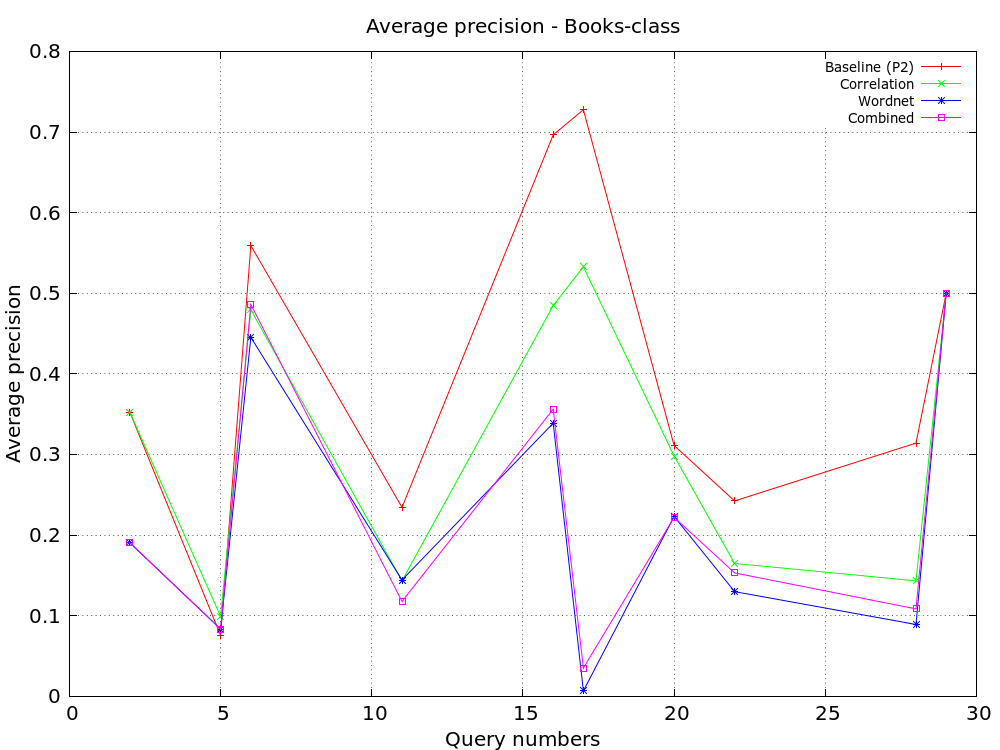
\includegraphics[scale = 0.4]{books_avg}
\end{center}

\begin{center}
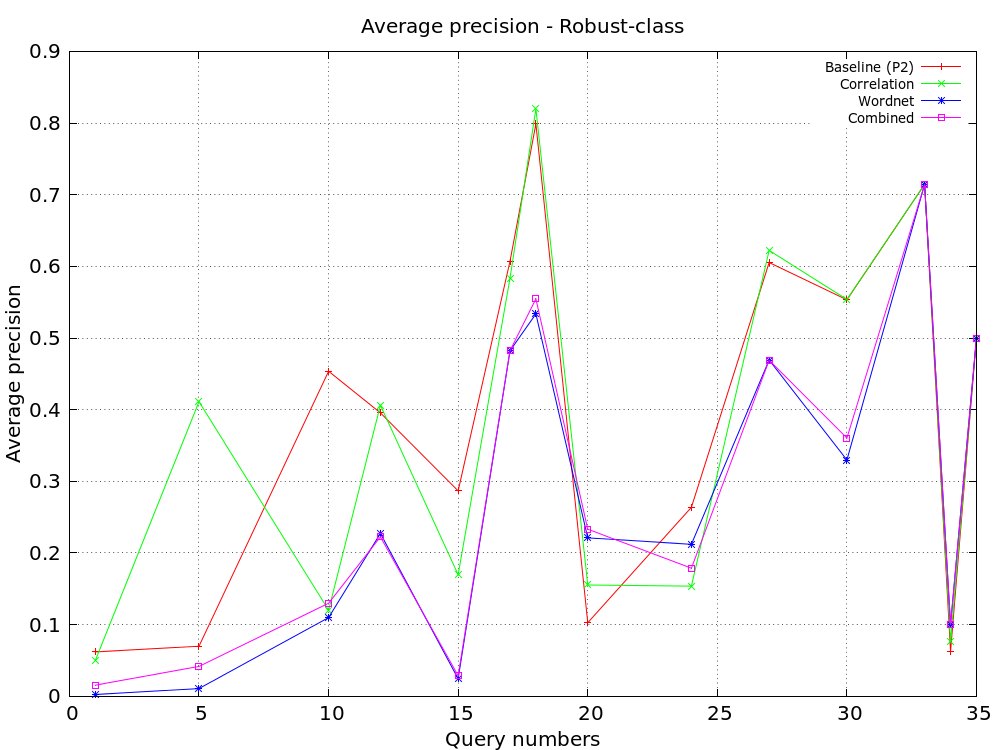
\includegraphics[scale = 0.4]{robust-class_avg}
\end{center}

\begin{center}
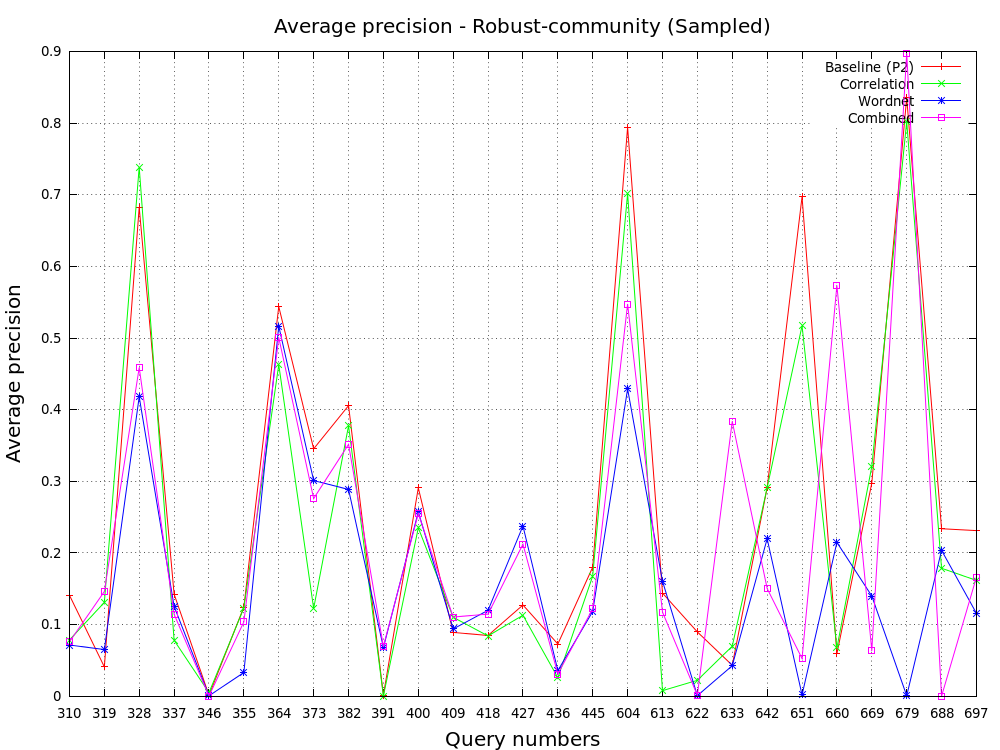
\includegraphics[scale = 0.4]{sampled-robust-comm_avg}
\end{center}

From the above plots valid conclusions can be drawn from the robust04 query results. We notice that the graphs for co-occurence based thesaurus queries and the baseline are actually almost similar, so from this we can understand that the over-all mean average precision is less because of the queries and the collection as such and the expanded queries perform as good or as poorly as the original queries. The mean average precision is less because the bad precision scores get cumulated and bring the average precision down.

\paragraph{}
For the rest of the measures, the plots for the TREC Robust dataset the only ones added because interesting conclusions can be drawn from them.

\subsection*{Precision at 10}
\begin{center}
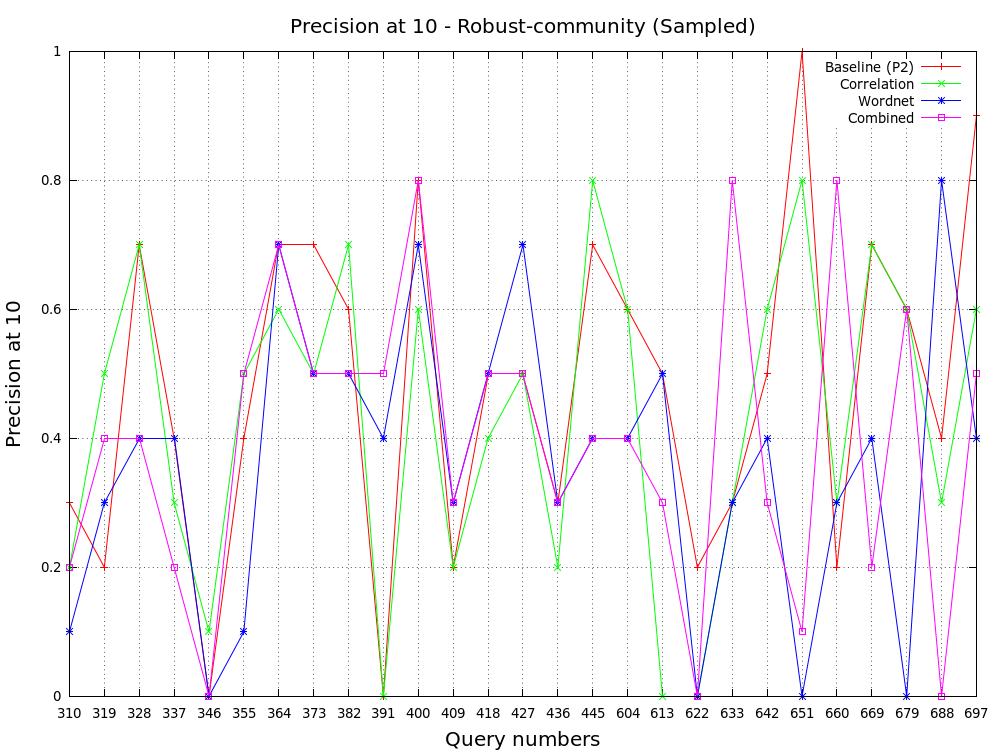
\includegraphics[scale = 0.4]{sampled-robust-comm_prec10}
\end{center}

The above graph shows that the co-occurrence thesaurus has a decent performance when you compare the average precision values and its precision at 10 values are better than the other two thesauri (Of course the baseline still performs better) This means that the queries expanded produces good results higher up in the ranked list but the precision decreases as more documents are retrieved.  

\subsection*{NDCG at 10}
\begin{center}
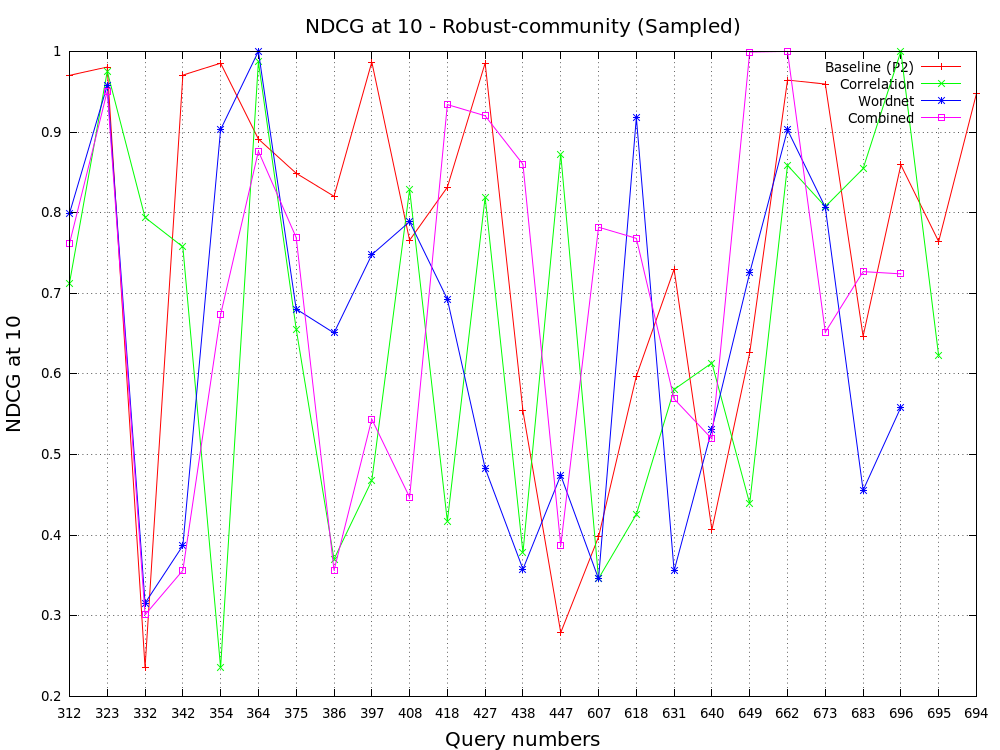
\includegraphics[scale = 0.4]{sampled-robust-comm_ndcg10}
\end{center}

The above graph is interesting and gives an overall picture of how the NDCGs are but concrete conclusions cannot be drawn from then, this made me lookup the average NDCGs for all the thesauri. Again, this data is from TRECRobust because I believe conclusions drawn from that data set can be generalized.

\begin{itemize}
\item Baseline: 0.6889
\item Co-occurrence: 0.6248
\item Combined: 0.5966
\item Wordnet: 0.6045
\end{itemize}

From the above numbers we can note that again it's the Co-occurrence thesaurus which performs the best out of the thesauri. 

\subsection*{...and finally} 
The results obtained is different from what is claimed in the paper, and this could be because, the dataset used was different and also because to help with computation times the words in the top 50 documents in the ranked list was used for similarity computations. 
\chapter{Conclusion and Future work}

Though in theory thesaurus-based query expansion should provide good results, in practice from the above experiments that likely is not the case. Some expanded queries are good. For example the wordnet based thesaurus expanded ``Beethoven's birthplace" to ``Beethoven birthplace origin sources composer" and the co-occurrence thesaurus expanded ``Best retirement country" to ``best retirement country  two pension project" which make sense. However most queries turn out to be something like ``brazil forest industry" becoming ``brazil forest industry woods timberland  manufactures" where in the expansion makes no sense. Combining evidence from various thesauri also does not make query expansion better.

Some takeaways:
\begin{itemize}
\item In all of these approaches, the sense of the query is not determined by the entire query as a whole. The thesaurus based approaches consider queries as bags of words each independent of each other.
\item  Thesaurus is a global model that is not related to the query, if a word is expanded with a synonym the resulting connotation might not be exactly appropriate.
\end{itemize}
 
An extension of the work can be query weighting. Query weighting has to be done in order to expand the query words and not give equal importance to the original query words and the words added as a part of query expansion. 

Also, instead of considering a query as a bag of words, queries as a whole can be used and a set of words which is synonymous with the query as a whole can be used for expansion.

\begin{thebibliography}{1}
\bibitem{wiki} \url{http://en.wikipedia.org/wiki/Query_expansion}
\bibitem{paper} \url{http://www.iro.umontreal.ca/~nie/IFT6255/mandala99combining.pdf}
\bibitem{textblob} \url{http://textblob.readthedocs.org/en/dev/}
\bibitem{galago} \url{http://www.lemurproject.org/galago.php}
\bibitem{ir} \url{en.wikipedia.org/wiki/Information_retrieval}
\bibitem{ndcg} \url{http://www.kaggle.com/wiki/NormalizedDiscountedCumulativeGain}
\end{thebibliography}



\end{document}